%!TEX root = mainfile.tex

\subsection{Observing Strategy for Redshift 8.5--10} % (fold)
\label{sub:using_euclid_for_a_survey_of_edshift_8_54_to_10_1}
	Due to its large field of view, Euclid space telescope will be useful for studying a large number of galaxies, however it has been found to be limited by its filters to providing colour information only for those objects between redshift 8.5 and 10, Section~\ref{sec:Photometry_Colour}. The Euclid survey as described in Section~\ref{sub:euclid} is planned to take approximately six years, but this will only reach a magnitude of 26. It was investigated what galaxies the telescope would be able to observe if the magnitude limit was increased, and the results are shown in Table~\ref{tab:filters_for_particular_redshift_galaxies}.

	It must be noted that the program results predict different numbers of galaxies than the Euclid documentation. The prediction group's program is the data on which the following calculations are based. The survey method adopted for this project would also be different from that detailed by the Euclid ``red book''; rather than revisiting the same patch of sky infrequently, the aim would be to stare continuously at a particular point until the required depth was met. No wide survey is required for this project since the galaxies at the high redshifts being studied all have faint magnitudes. This will take a considerable length of time to see; hence a wide survey at such depths is implausible.

	Table~\ref{tab:filters_for_particular_redshift_galaxies} shows the number of galaxies observable for survey times of 0.1, 0.2, and 0.5\,million seconds. The number of galaxies that would be observed at different magnitudes is presented, and the table also displays the time taken for 1\,FoV, and the number of galaxies in that field of view for each magnitude. The red number indicates how many FoVs were possible given the set total observing time. N/A indicates that there were either no galaxies at this magnitude, or that the time taken to get to this magnitude was larger than the intended total survey time.
	\begin{table}[htbp]
		\begin{center}
			\begin{tabular}{c|c|c|c|c|c}
				\multirow{2}{*}{Magnitude}	&Time for	&Number of	&\multicolumn{3}{|c}{Galaxies in total observing time of:}\\
					\cline{4-6}
					&1\,FoV (\si{\second})	&galaxies in 1 FoV	&0.1 mil	&0.2 mil	&0.5 mil\\
				\hline \hline
				27		&\num{2.09e3}	&None	&N/A	&N/A	&N/A\\
				28		&\num{7.67e3}	&0.052	&0.6 (13)	&1.35 (26)	&3.38 (65)\\
				28.5	&\num{1.65e4}	&1.26	&7.56 (6)	&15.12 (12)	&37.8 (30)\\
				29		&\num{3.78e4}	&12.55	&25.1 (2)	&62.75 (5)	&163.15 (13)\\
				29.5	&\num{9.90e4}	&69.37	&69.37 (1)	&138.74 (2)	&346.85 (5)\\
				30		&\num{2.25e5}	&256.23	&N/A		&N/A		&512.46 (2)\\
				31		&\num{1.39e6}	&1653.35	&N/A	&N/A		&N/A
			\end{tabular}
		\end{center}
		\caption{Data highlighting which filters would be useful for observing particular redshift galaxies\cite{Galactic_Astronomy_Binney_Merrifield}}
		\label{tab:filters_for_particular_redshift_galaxies}
	\end{table}

	\begin{figure}[htbp]
		\centering
			\begingroup\endlinechar=-1
				\resizebox{0.8\textwidth}{!}{%
					% GNUPLOT: LaTeX picture with Postscript
\begingroup
  \makeatletter
  \providecommand\color[2][]{%
    \GenericError{(gnuplot) \space\space\space\@spaces}{%
      Package color not loaded in conjunction with
      terminal option `colourtext'%
    }{See the gnuplot documentation for explanation.%
    }{Either use 'blacktext' in gnuplot or load the package
      color.sty in LaTeX.}%
    \renewcommand\color[2][]{}%
  }%
  \providecommand\includegraphics[2][]{%
    \GenericError{(gnuplot) \space\space\space\@spaces}{%
      Package graphicx or graphics not loaded%
    }{See the gnuplot documentation for explanation.%
    }{The gnuplot epslatex terminal needs graphicx.sty or graphics.sty.}%
    \renewcommand\includegraphics[2][]{}%
  }%
  \providecommand\rotatebox[2]{#2}%
  \@ifundefined{ifGPcolor}{%
    \newif\ifGPcolor
    \GPcolortrue
  }{}%
  \@ifundefined{ifGPblacktext}{%
    \newif\ifGPblacktext
    \GPblacktexttrue
  }{}%
  % define a \g@addto@macro without @ in the name:
  \let\gplgaddtomacro\g@addto@macro
  % define empty templates for all commands taking text:
  \gdef\gplbacktext{}%
  \gdef\gplfronttext{}%
  \makeatother
  \ifGPblacktext
    % no textcolor at all
    \def\colorrgb#1{}%
    \def\colorgray#1{}%
  \else
    % gray or color?
    \ifGPcolor
      \def\colorrgb#1{\color[rgb]{#1}}%
      \def\colorgray#1{\color[gray]{#1}}%
      \expandafter\def\csname LTw\endcsname{\color{white}}%
      \expandafter\def\csname LTb\endcsname{\color{black}}%
      \expandafter\def\csname LTa\endcsname{\color{black}}%
      \expandafter\def\csname LT0\endcsname{\color[rgb]{1,0,0}}%
      \expandafter\def\csname LT1\endcsname{\color[rgb]{0,1,0}}%
      \expandafter\def\csname LT2\endcsname{\color[rgb]{0,0,1}}%
      \expandafter\def\csname LT3\endcsname{\color[rgb]{1,0,1}}%
      \expandafter\def\csname LT4\endcsname{\color[rgb]{0,1,1}}%
      \expandafter\def\csname LT5\endcsname{\color[rgb]{1,1,0}}%
      \expandafter\def\csname LT6\endcsname{\color[rgb]{0,0,0}}%
      \expandafter\def\csname LT7\endcsname{\color[rgb]{1,0.3,0}}%
      \expandafter\def\csname LT8\endcsname{\color[rgb]{0.5,0.5,0.5}}%
    \else
      % gray
      \def\colorrgb#1{\color{black}}%
      \def\colorgray#1{\color[gray]{#1}}%
      \expandafter\def\csname LTw\endcsname{\color{white}}%
      \expandafter\def\csname LTb\endcsname{\color{black}}%
      \expandafter\def\csname LTa\endcsname{\color{black}}%
      \expandafter\def\csname LT0\endcsname{\color{black}}%
      \expandafter\def\csname LT1\endcsname{\color{black}}%
      \expandafter\def\csname LT2\endcsname{\color{black}}%
      \expandafter\def\csname LT3\endcsname{\color{black}}%
      \expandafter\def\csname LT4\endcsname{\color{black}}%
      \expandafter\def\csname LT5\endcsname{\color{black}}%
      \expandafter\def\csname LT6\endcsname{\color{black}}%
      \expandafter\def\csname LT7\endcsname{\color{black}}%
      \expandafter\def\csname LT8\endcsname{\color{black}}%
    \fi
  \fi
  \setlength{\unitlength}{0.0500bp}%
  \begin{picture}(7200.00,4320.00)%
    \gplgaddtomacro\gplbacktext{%
      \put(747,595){\makebox(0,0)[r]{\strut{} 0}}%
      \put(747,1182){\makebox(0,0)[r]{\strut{} 100}}%
      \put(747,1768){\makebox(0,0)[r]{\strut{} 200}}%
      \put(747,2355){\makebox(0,0)[r]{\strut{} 300}}%
      \put(747,2942){\makebox(0,0)[r]{\strut{} 400}}%
      \put(747,3528){\makebox(0,0)[r]{\strut{} 500}}%
      \put(747,4115){\makebox(0,0)[r]{\strut{} 600}}%
      \put(849,409){\makebox(0,0){\strut{} 27.5}}%
      \put(1856,409){\makebox(0,0){\strut{} 28}}%
      \put(2864,409){\makebox(0,0){\strut{} 28.5}}%
      \put(3871,409){\makebox(0,0){\strut{} 29}}%
      \put(4878,409){\makebox(0,0){\strut{} 29.5}}%
      \put(5886,409){\makebox(0,0){\strut{} 30}}%
      \put(6893,409){\makebox(0,0){\strut{} 30.5}}%
      \csname LTb\endcsname%
      \put(144,2355){\rotatebox{-270}{\makebox(0,0){\strut{}Number of Galaxies}}}%
      \csname LTb\endcsname%
      \put(3871,130){\makebox(0,0){\strut{}Magnitude ($M$)}}%
      \put(3871,4022){\makebox(0,0){\strut{}}}%
    }%
    \gplgaddtomacro\gplfronttext{%
      \csname LTb\endcsname%
      \put(2178,3729){\makebox(0,0)[r]{\strut{}\SI{0.1e6}{\second}}}%
      \csname LTb\endcsname%
      \put(2178,3543){\makebox(0,0)[r]{\strut{}\SI{0.2e6}{\second}}}%
      \csname LTb\endcsname%
      \put(2178,3357){\makebox(0,0)[r]{\strut{}\SI{0.5e6}{\second}}}%
    }%
    \gplbacktext
    \put(0,0){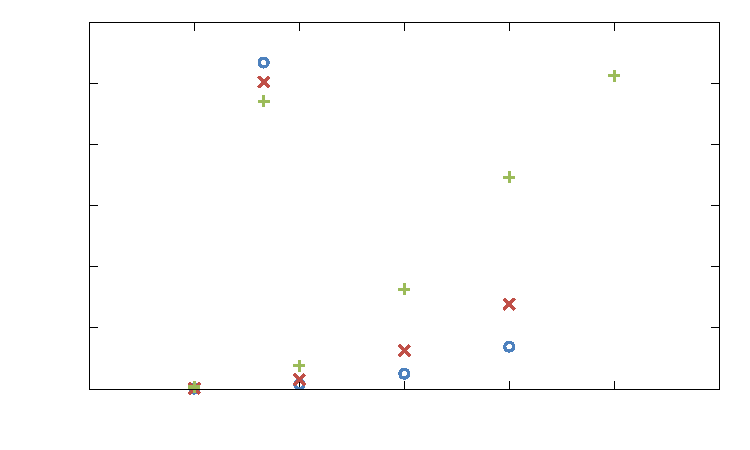
\includegraphics{GRAPH_Mag_vs_galaxies_in_time_Euclid}}%
    \gplfronttext
  \end{picture}%
\endgroup

				}\endgroup
		\caption{Number of galaxies expected for different magnitudes, given set overall observing time for the Euclid Space Telescope.\label{fig:galaxies_expected_EST}}
	\end{figure}

	For increasing magnitudes, the total number of objects given a total observing time was found to increase within the range \numrange{27}{31}. A survey of \SI{0.1e6}{\second} for each filter yielded best results at a magnitude of 29.5. Around 70 galaxies between a redshift of 8.5 and 10 would be expected. However this would involve one pointing of the telescope, which would lead to a large uncertainty on the number due to cosmic variance.
	\begin{figure}[htbp]
		\centering
			\begingroup\endlinechar=-1
				\resizebox{0.8\textwidth}{!}{%
					% GNUPLOT: LaTeX picture with Postscript
\begingroup
  \makeatletter
  \providecommand\color[2][]{%
    \GenericError{(gnuplot) \space\space\space\@spaces}{%
      Package color not loaded in conjunction with
      terminal option `colourtext'%
    }{See the gnuplot documentation for explanation.%
    }{Either use 'blacktext' in gnuplot or load the package
      color.sty in LaTeX.}%
    \renewcommand\color[2][]{}%
  }%
  \providecommand\includegraphics[2][]{%
    \GenericError{(gnuplot) \space\space\space\@spaces}{%
      Package graphicx or graphics not loaded%
    }{See the gnuplot documentation for explanation.%
    }{The gnuplot epslatex terminal needs graphicx.sty or graphics.sty.}%
    \renewcommand\includegraphics[2][]{}%
  }%
  \providecommand\rotatebox[2]{#2}%
  \@ifundefined{ifGPcolor}{%
    \newif\ifGPcolor
    \GPcolortrue
  }{}%
  \@ifundefined{ifGPblacktext}{%
    \newif\ifGPblacktext
    \GPblacktexttrue
  }{}%
  % define a \g@addto@macro without @ in the name:
  \let\gplgaddtomacro\g@addto@macro
  % define empty templates for all commands taking text:
  \gdef\gplbacktext{}%
  \gdef\gplfronttext{}%
  \makeatother
  \ifGPblacktext
    % no textcolor at all
    \def\colorrgb#1{}%
    \def\colorgray#1{}%
  \else
    % gray or color?
    \ifGPcolor
      \def\colorrgb#1{\color[rgb]{#1}}%
      \def\colorgray#1{\color[gray]{#1}}%
      \expandafter\def\csname LTw\endcsname{\color{white}}%
      \expandafter\def\csname LTb\endcsname{\color{black}}%
      \expandafter\def\csname LTa\endcsname{\color{black}}%
      \expandafter\def\csname LT0\endcsname{\color[rgb]{1,0,0}}%
      \expandafter\def\csname LT1\endcsname{\color[rgb]{0,1,0}}%
      \expandafter\def\csname LT2\endcsname{\color[rgb]{0,0,1}}%
      \expandafter\def\csname LT3\endcsname{\color[rgb]{1,0,1}}%
      \expandafter\def\csname LT4\endcsname{\color[rgb]{0,1,1}}%
      \expandafter\def\csname LT5\endcsname{\color[rgb]{1,1,0}}%
      \expandafter\def\csname LT6\endcsname{\color[rgb]{0,0,0}}%
      \expandafter\def\csname LT7\endcsname{\color[rgb]{1,0.3,0}}%
      \expandafter\def\csname LT8\endcsname{\color[rgb]{0.5,0.5,0.5}}%
    \else
      % gray
      \def\colorrgb#1{\color{black}}%
      \def\colorgray#1{\color[gray]{#1}}%
      \expandafter\def\csname LTw\endcsname{\color{white}}%
      \expandafter\def\csname LTb\endcsname{\color{black}}%
      \expandafter\def\csname LTa\endcsname{\color{black}}%
      \expandafter\def\csname LT0\endcsname{\color{black}}%
      \expandafter\def\csname LT1\endcsname{\color{black}}%
      \expandafter\def\csname LT2\endcsname{\color{black}}%
      \expandafter\def\csname LT3\endcsname{\color{black}}%
      \expandafter\def\csname LT4\endcsname{\color{black}}%
      \expandafter\def\csname LT5\endcsname{\color{black}}%
      \expandafter\def\csname LT6\endcsname{\color{black}}%
      \expandafter\def\csname LT7\endcsname{\color{black}}%
      \expandafter\def\csname LT8\endcsname{\color{black}}%
    \fi
  \fi
  \setlength{\unitlength}{0.0500bp}%
  \begin{picture}(7200.00,4320.00)%
    \gplgaddtomacro\gplbacktext{%
      \put(747,595){\makebox(0,0)[r]{\strut{}-100}}%
      \put(747,947){\makebox(0,0)[r]{\strut{} 0}}%
      \put(747,1299){\makebox(0,0)[r]{\strut{} 100}}%
      \put(747,1651){\makebox(0,0)[r]{\strut{} 200}}%
      \put(747,2003){\makebox(0,0)[r]{\strut{} 300}}%
      \put(747,2355){\makebox(0,0)[r]{\strut{} 400}}%
      \put(747,2707){\makebox(0,0)[r]{\strut{} 500}}%
      \put(747,3059){\makebox(0,0)[r]{\strut{} 600}}%
      \put(747,3411){\makebox(0,0)[r]{\strut{} 700}}%
      \put(747,3763){\makebox(0,0)[r]{\strut{} 800}}%
      \put(747,4115){\makebox(0,0)[r]{\strut{} 900}}%
      \put(849,409){\makebox(0,0){\strut{} 27.5}}%
      \put(1856,409){\makebox(0,0){\strut{} 28}}%
      \put(2864,409){\makebox(0,0){\strut{} 28.5}}%
      \put(3871,409){\makebox(0,0){\strut{} 29}}%
      \put(4878,409){\makebox(0,0){\strut{} 29.5}}%
      \put(5886,409){\makebox(0,0){\strut{} 30}}%
      \put(6893,409){\makebox(0,0){\strut{} 30.5}}%
      \csname LTb\endcsname%
      \put(144,2355){\rotatebox{-270}{\makebox(0,0){\strut{}Number of Galaxies}}}%
      \csname LTb\endcsname%
      \put(3871,130){\makebox(0,0){\strut{}Magnitude ($M$)}}%
      \put(3871,4022){\makebox(0,0){\strut{}}}%
    }%
    \gplgaddtomacro\gplfronttext{%
      \csname LTb\endcsname%
      \put(2178,3670){\makebox(0,0)[r]{\strut{}\SI{0.1e6}{\second}}}%
      \csname LTb\endcsname%
      \put(2178,3484){\makebox(0,0)[r]{\strut{}\SI{0.2e6}{\second}}}%
      \csname LTb\endcsname%
      \put(2178,3298){\makebox(0,0)[r]{\strut{}\SI{0.5e6}{\second}}}%
    }%
    \gplbacktext
    \put(0,0){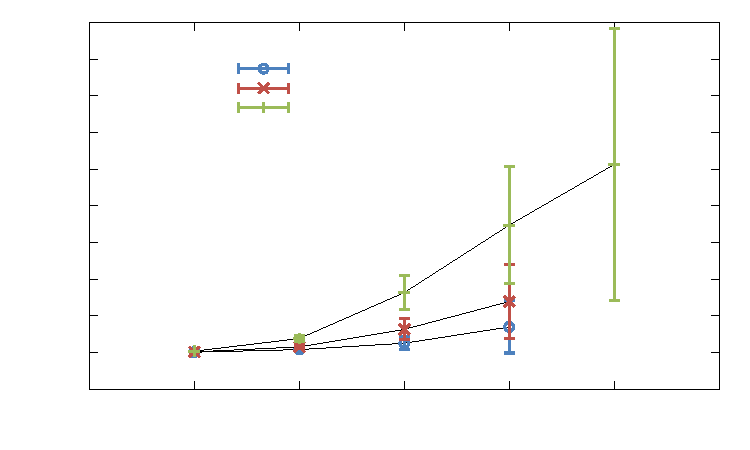
\includegraphics{GRAPH_Mag_vs_galaxies_in_time_Euclid_errors}}%
    \gplfronttext
  \end{picture}%
\endgroup

				}\endgroup
		\caption{Number of galaxies expected for different magnitudes, given set overall observing time for the Euclid Telescope.\label{fig:galaxies_expected_Euclid}}
	\end{figure}

	The alternative option was to double the survey time to \SI{0.2e6}{\second}, which yielded 63 galaxies at a magnitude of 29.0, and increasing the number of pointings (and survey area) by a factor of five, thus reducing the cosmic variance. For the same time, there was also the option of observing around 140 galaxies down to a magnitude of 29.5, with 2 pointings of the telescope.

	In order to keep time to a minimum, it was decided that the \SI{0.1e6}{\second} option was best, as each galaxy needs to be observed in three filters, and subsequently confirmed by spectroscopy. The multi-band photometry approximately triples the \SI{0.1e6}{\second} to \SI{0.3e6}{\second}. Added to this, overhead times extend the time further as the telescope will need to be read out. As an approximation, this increases the total time taken to do photometry to around \SI{0.6e6}{\second}, or 7\,days continuous viewing. The telescope is assumed to be operational for 18\,hours a day, meaning that the shortest time over which this survey could be done is around ten days, not including spectroscopy.
% subsection using_euclid_for_a_survey_of_edshift_8_54_to_10_1 (end)
